%!TEX root = ./lec04_access_methods.tex

%
% -------------------------------------------------------------------------------------------------------
%
\begin{frame}{Extensible hashing}

Two ingredients:

\begin{enumerate}[label=(\arabic*)]
\item keep a \textbf{directory} mapping \emph{logical buckets} into physical buckets (i.e., disk blocks)

\item the hash function computes a sequence of $k$ bits (e.g., $k=64$); but only the \alert{first $i$} bits are used to number the logical buckets
\end{enumerate}

\textbf{Example:} $k=4$ and $i=1$

\begin{center}
\setcounter{tIdCnt}{0}
\scalebox{0.75}{
\begin{tikzpicture}
\directory{d}{0}{-1}{1};
\extensibleHashBlock{b0}{2}{0}{1}
\extensibleHashBlock{b1}{2}{-2}{1}
\hashLink{d}{0}{b0}
\hashLink{d}{1}{b1}
\dynamicHashBlockEntry{b0}{0}{0110}{$t_1$}
\dynamicHashBlockEntry{b1}{0}{1011}{$t_2$}
\dynamicHashBlockEntry{b0}{1}{0011}{$t_3$}
\end{tikzpicture}}
\end{center}
\end{frame}


%
% -------------------------------------------------------------------------------------------------------
%
\begin{frame}{Insertion with Extensible Hashing}

Like before, every new tuple $t_i$ goes into bucket $h(t_i)$.

\vskip1em

\textbf{Example:} insert $t_4$ with $h(t_4) = 1001$. 

\vskip1em

\begin{center}
\setcounter{tIdCnt}{0}
\scalebox{0.75}{
\begin{tikzpicture}
\extensibleHashBlock{b0}{2}{0}{1}
\extensibleHashBlock{b1}{2}{-2}{1}
\dynamicHashBlockEntry{b0}{0}{0110}{$t_1$}
\dynamicHashBlockEntry{b1}{0}{1011}{$t_2$}
\dynamicHashBlockEntry{b0}{1}{0011}{$t_3$}


\only<1-2|handout:1>{
	\directory{d}{0}{-1}{1};
	\hashLink{d}{0}{b0}
	\hashLink{d}{1}{b1}
}

\only<2|handout:1>{
	\dynamicHashBlockEntry{b1}{1}{1001}{$t_4$};

	\node (0) at (2.25,-2.8) [thick,color=red,draw,rectangle,minimum height = 1.25em,minimum width = 1.25em] {};
	\node (1) at (-0.45,-1.8) [thick,color=red,draw,rectangle,minimum height = 1.25em,minimum width = 1.25em] {};
	\draw [->,thick, color=red] (0) -- (1);
}
\end{tikzpicture}}
\end{center}
\end{frame}


%
% -------------------------------------------------------------------------------------------------------
%
\begin{frame}

Inserting a tuple into a bucket that is already full forces the \textbf{directory} to grow, by \framebox{increasing \alert{$i$}}.


\vskip1em

\textbf{Example:} insert $t_5$ with $h(t_5) = 0100$. 

\vskip1em

\begin{center}
\setcounter{tIdCnt}{0}
\scalebox{0.75}{
\begin{tikzpicture}
	\extensibleHashBlock{b1}{2}{-4}{1}
	\dynamicHashBlockEntry{b1}{0}{1011}{$t_2$}
	\dynamicHashBlockEntry{b1}{1}{1001}{$t_4$}

\only<1|handout:0>{
	\directory{d}{0}{-1}{1};
	\extensibleHashBlock{b0}{2}{0}{1}	
	\hashLink{d}{0}{b0}
	\hashLink{d}{1}{b1}
	\dynamicHashBlockEntry{b0}{0}{0110}{$t_1$}
	\dynamicHashBlockEntry{b0}{1}{0011}{$t_3$}
}

\only<2-3|handout:1>{
	\directory{d}{0}{-2}{2};
	\extensibleHashBlock{b00}{2}{0}{2}
	\extensibleHashBlock{b01}{2}{-2}{2}

	\hashLink{d}{0}{b00}
	\hashLink{d}{1}{b01}
	\hashLink{d}{2}{b1}
	\hashLink{d}{3}{b1}

	\dynamicHashBlockEntry{b01}{0}{0110}{$t_1$}
	\dynamicHashBlockEntry{b01}{1}{0100}{$t_5$}
	\dynamicHashBlockEntry{b00}{0}{0011}{$t_3$}
}

\only<3|handout:0>{
	\coordinate [left= 1cm of b00] (0) ;
	\draw [->,very thick,color=blue] ([yshift=1em]0) -- ([yshift=5pt]b00.north west);

	\coordinate [left= 1cm of b01] (1) ;
	\draw [->,very thick,color=blue] ([yshift=1em]1) -- ([yshift=5pt]b01.north west);

	\draw [color=red,decorate,decoration={brace,amplitude=5pt,raise=8pt},yshift=0pt]
		(-0.5,-4.2) -- (-0.5,-3) node [midway,xshift=-2.5cm] {
	\begin{minipage}{3.5cm}\baselineskip=0.75\baselineskip \centering
		two logical buckets sharing the same physical bucket
	\end{minipage}
		};
}
\end{tikzpicture}}
\end{center}
\end{frame}


%
% -------------------------------------------------------------------------------------------------------
%
\begin{frame}

\textbf{Example:} insert $t_6$ with $h(t_6) = 0100$. 

\vskip1em

\begin{center}
\setcounter{tIdCnt}{0}
\scalebox{0.75}{
\begin{tikzpicture}
	\extensibleHashBlock{b00}{2}{0}{2}
	\extensibleHashBlock{b1}{2}{-6}{1}
	\dynamicHashBlockEntry{b1}{0}{1011}{$t_2$}
	\dynamicHashBlockEntry{b1}{1}{1001}{$t_4$}
	\dynamicHashBlockEntry{b00}{0}{0011}{$t_3$}

\only<1|handout:0>{
	\directory{d}{0}{-2}{2};

	\extensibleHashBlock{b01}{2}{-2}{2}

	\hashLink{d}{0}{b00}
	\hashLink{d}{1}{b01}
	\hashLink{d}{2}{b1}
	\hashLink{d}{3}{b1}

	\dynamicHashBlockEntry{b01}{0}{0110}{$t_1$}
	\dynamicHashBlockEntry{b01}{1}{0100}{$t_5$}
}

\only<2|handout:1>{
	\directory{d}{0}{-2.5}{3};
	\extensibleHashBlock{b010}{2}{-2}{3}
	\extensibleHashBlock{b011}{2}{-4}{3}

	\hashLink{d}{0}{b00}
	\hashLink{d}{1}{b00}
	\hashLink{d}{2}{b010}
	\hashLink{d}{3}{b011}
	\hashLink{d}{4}{b1}
	\hashLink{d}{5}{b1}
	\hashLink{d}{6}{b1}
	\hashLink{d}{7}{b1}

	\dynamicHashBlockEntry{b011}{0}{0110}{$t_1$}
	\dynamicHashBlockEntry{b010}{0}{0100}{$t_5$}
	\dynamicHashBlockEntry{b010}{1}{0100}{$t_6$}
}
\end{tikzpicture}}
\end{center}
\end{frame}

\newsavebox{\dynamicHashingExample}
\savebox{\dynamicHashingExample}{
\begin{tikzpicture}
	\directory{d}{0}{-2.5}{3};
	\extensibleHashBlock{b010}{2}{-2}{3}
	\extensibleHashBlock{b011}{2}{-4}{3}
	\extensibleHashBlock{b00}{2}{0}{2}
	\extensibleHashBlock{b1}{2}{-6}{1}

	\hashLink{d}{0}{b00}
	\hashLink{d}{1}{b00}
	\hashLink{d}{2}{b010}
	\hashLink{d}{3}{b011}
	\hashLink{d}{4}{b1}
	\hashLink{d}{5}{b1}
	\hashLink{d}{6}{b1}
	\hashLink{d}{7}{b1}

	\dynamicHashBlockEntry{b1}{0}{1011}{$t_2$}
	\dynamicHashBlockEntry{b1}{1}{1001}{$t_4$}
	\dynamicHashBlockEntry{b00}{0}{0011}{$t_3$}
	\dynamicHashBlockEntry{b011}{0}{0110}{$t_1$}
	\dynamicHashBlockEntry{b010}{0}{0100}{$t_5$}
	\dynamicHashBlockEntry{b010}{1}{0100}{$t_6$}
\end{tikzpicture}}

%
% -------------------------------------------------------------------------------------------------------
%
\begin{frame}{Deletions with Extensible Hashing}

Deletions are only an issue if they cause a \textbf{physical} bucket to become empty.

\textbf{Example:} delete tuple $t_1$ with $h(t_1)=0110$.

\vskip1em

\begin{columns}[onlytextwidth]
\begin{column}{0.6\textwidth}
\textbf{Option 1:} \alert{merge logical buckets} (010 and 011 in this case); \alert{shrink the directory} (decrease $i$) if needed\footnotemark.

\vskip1em

\textbf{Option 2:} put a ``tombstone'' mark (
\includegraphics[height=1em]{images/RIP.pdf}) in place of $t_1$. Re-build table when database goes offline for maintenance.
\end{column}
\begin{column}{0.3\textwidth}
\scalebox{0.5}{\usebox\dynamicHashingExample}
\end{column}
\end{columns}
\vskip1em

\footnotetext{Not all deletions lead to shrinking the directory. For example, there would be no shrinking if logical buckets 000 and 001 were on separate physical buckets.}
\end{frame}

%
% -------------------------------------------------------------------------------------------------------
%
\begin{frame}{Too Many Collisions can Break Extensible Hashing}

\textbf{Example:} how to handle the insertion of $t_7$ with $h(t_7)=0100$? 

When more tuples hash to the same bucket than a physical bucket can fit, further growing the directory doesn't help.

\vskip1em

\begin{columns}[onlytextwidth]
\begin{column}{0.6\textwidth}
\textbf{Option 1:} start an \alert{overflow chain} on the block with $t_5$ and $t_6$.

\vskip1em

\textbf{Option 2:} add a level of indirection with ``bucket files''\footnotemark as was done for secondary indexes (slide~\ref{bucket_files_secondary_indexes}). This increases I/O cost.
\end{column}
\begin{column}{0.3\textwidth}
\scalebox{0.5}{\usebox\dynamicHashingExample}
\end{column}
\end{columns}

\footnotetext{Not to be confused with the ``hashing buckets''.}

\end{frame}

%
% -------------------------------------------------------------------------------------------------------
%
\begin{frame}{Extensible Hashing: Summary}

\textbf{Pros:}\\
 - without duplicates, physical buckets are always 1 disk block\\
 - all operations require $O(1)$ I/O (if directory can fit in memory)\\
 - ``file'' on disk grows one block at a time

\textbf{Cons:}\\
 - need to keep directory in memory (or do more I/O)\\
 - directory grows exponentially
 
\vskip1em

\textbf{Worst problem of extensible hashing}: a ``bad'' hash function can cause the directory to grow very big (very fast). Suppose $k=32$ and the number of tuples per bucket is 2 (as in the running example). If there are 3 tuples whose hash values disagree on their $20^{\mathit{th}}$ bit, the directory will grow to $2^{20}$ entries to hold them.
\end{frame}

%
% -------------------------------------------------------------------------------------------------------
%